\SourcePage{GELFAND-P001228}{unlabelled}
\(\alpha_+,\alpha_-\), \(\alpha_+\alpha_-=-2\).
\Unclear{GELFAND-P001228}{equality-mark}{Мелкая помета над знаком равенства не разобрана.}
\end{GelfandAdjacentEvidence}
\begin{GelfandAdjacentEvidence}{GELFAND-P001228}{2}

\begin{equation*}
\begin{aligned}
&\int_0^1
\prod_{\substack{i,j=1\\i<j}}^{n}(t_i-t_j)^{\alpha_+^2}
\prod_{\substack{n+1\le i,j\le n+m\\i<j}}(t_i-t_j)^{\alpha_-^2}
\left(\prod_{i=1}^{n+m}t_i\right)^\beta\\
&\qquad{}\cdot\prod_{\substack{1\le u\le n\\n+1\le v\le m+1}}(t_u-t_v)^{-2}\cdot\\
&\qquad{}\cdot\prod_{1\le i\le n}(z-t_i)^\gamma
\prod_{n+1\le i\le n+m}(z-t_i)^\delta\,dt_1\ldots dt_n.
\end{aligned}\tag{18}
\end{equation*}
\Unclear{GELFAND-P001228}{first-product-cancellation}{Между \(i,j=1\) и \(i<j\) под первым произведением зачёркнута запись. В ней видны штрихи, похожие на \(i\) и \(j\). Знак между ними неразборчив.}
\end{GelfandAdjacentEvidence}
\begin{GelfandAdjacentEvidence}{GELFAND-P001228}{3}

\Unclear{GELFAND-P001228}{mixed-product-cancellation}{Под двумя условиями смешанного произведения зачёркнут неразобранный знак.}
\end{GelfandAdjacentEvidence}
\begin{GelfandAdjacentEvidence}{GELFAND-P001228}{4}

\EvidenceBlock{GELFAND-P001228}{integral-index-mismatch}{Верхняя граница для \(v\) написана \(m+1\). Последний дифференциал написан \(dt_n\).}{Запись в рукописи.}
\end{GelfandAdjacentEvidence}
\begin{GelfandAdjacentEvidence}{GELFAND-P001228}{5}


В таком виде представляется 2-точечная корреляционная ф-я теории (конформной теории поля).

[зачёркнуто] Так получается [счетное?] число корреляц. ф-й.
\Unclear{GELFAND-P001228}{prose-cancellation}{Перед «Так» зачёркнуто слово, предположительно «Если».}
\end{GelfandAdjacentEvidence}
\begin{GelfandAdjacentEvidence}{GELFAND-P001228}{6}

\Unclear{GELFAND-P001228}{count-word}{Слово перед «число» предположительно читается «счетное». Конец «етное» различим, начальные штрихи неясны.}
\end{GelfandAdjacentEvidence}
\begin{GelfandAdjacentEvidence}{GELFAND-P001228}{7}


Реальные ф-и --- их аналит. продолж. на комплексные \(n\) и \(m\).

\uwave{Она наз. \(4^{\underline{\text{х}}}\) точечной} (хотя зав. только от \(z\)).

[Короткая черта вниз от \(z\)] [зачёркнуто] ангарм. отношение 4-ки точек на \(CP^1\).
\Unclear{GELFAND-P001228}{marginal-cancellation}{Перед «ангарм.» зачёркнуто слово, предположительно «она».}
\end{GelfandAdjacentEvidence}
\begin{GelfandAdjacentEvidence}{GELFAND-P001228}{8}

\EvidenceBlock{GELFAND-P001228}{correlation-order}{Вверху написано «2-точечная», ниже написано «\(4^{\underline{\text{х}}}\) точечной».}{Запись в рукописи.}
\end{GelfandAdjacentEvidence}



\Needspace{7\baselineskip}
\begin{GelfandAdjacentEvidence}{GELFAND-P001229}{1}
\SourcePage{GELFAND-P001229}{unlabelled}
\underline{\(11/\overline{\underline{\mathrm{XI}}}-85\) г.}\qquad
\underline{Сем. Гельфанда}

\underline{\underline{Вершик А.М.}}\qquad \underline{Топология пространств[а?] конфигураций.}
\Unclear{GELFAND-P001229}{title-word}{Отчётливо написано «пространств». Залитый последний знак предположительно читается «а». Справа от него видна отдельная точка.}
\end{GelfandAdjacentEvidence}
\begin{GelfandAdjacentEvidence}{GELFAND-P001229}{2}


\(1^{\circ}.\)
\SourceFigure{GELFAND-P001229}{grassmann-membership}{%
\par\smallskip
{\color{black}\begingroup\color{black}\GelfandFitDiagram{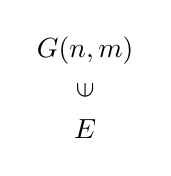
\begin{tikzpicture}
\node at (0,0) {\(G(n,m)\)};
\node[rotate=90] at (0,-.5) {\(\in\)};
\node at (0,-1) {\(E\)};
\end{tikzpicture}}\endgroup}\par\smallskip}
\end{GelfandAdjacentEvidence}
\begin{GelfandAdjacentEvidence}{GELFAND-P001229}{3}

\(e_1,\ldots,e_n\) --- базис в \(\mathbb R^n\)
\begin{equation*}
\tau_E=(Pe_1,\ldots,Pe_n)
\end{equation*}
Какова топ. страта в \(G(n,m)\), где \(\tau_E\) имеет заданный комбинат. тип?

\(2^{\circ}.\) Комбинат. теория выпуклых многогранников в \(\mathbb R^n\).

2 многогранника \(V_1,V_2\) с упорядоч. (занумер.) вершинами (\(n\) штук)
[зачёркнуто] имеют одинак. комбинат. тип, если грани соответствуют друг другу.
\Incomplete{GELFAND-P001229}{cancelled-type}{Зачёркнутый фрагмент после «\(n\) штук» не разобран.}
\end{GelfandAdjacentEvidence}
\begin{GelfandAdjacentEvidence}{GELFAND-P001229}{4}


Грассманизация задачи.

В \(\mathbb R^n\) рассм. подпр-во (\(m\)-мерное) \(E\)
\begin{equation*}
S=\omega(e_1,\ldots,e_n)\quad\text{--- симплекс}
\end{equation*}
\EvidenceBlock{GELFAND-P001229}{simplex-symbol}{После знака равенства написано \(\omega\).}{Запись в рукописи.}
\end{GelfandAdjacentEvidence}
\begin{GelfandAdjacentEvidence}{GELFAND-P001229}{5}

Проекция \(S\) на \(E\) --- многогранник (выпуклый)

\underline{Упр.:} получ. комбинаторно любой многогранник разм. \(m\) с \(n\) вершинами

На \(G(n,m)\) рассм. разбиение на подмн-ва, где несомые подпр-вом многогранники комбинаторно эквивалентны.
\EvidenceBlock{GELFAND-P001229}{subspace-abbreviation}{После «несомые» написано «подпр-вом».}{Запись в рукописи.}
\end{GelfandAdjacentEvidence}
\begin{GelfandAdjacentEvidence}{GELFAND-P001229}{6}


Какова топология этих кусков?

\(3^{\circ}.\)
\SourceFigure{GELFAND-P001229}{matrix-hatching}{%
\par\smallskip
{\color{black}\(\begin{array}{c}
\left(\begin{array}{@{}ccc@{}}
x_{11}&\cdots&x_{1n}\\
x_{21}&\cdots&x_{2n}\\
x_{31}&\cdots&x_{3n}\\
\hline
\multicolumn{3}{c}{\text{\tikz[x=.65cm,y=.40cm]{
\draw (0,.02)--(.37,.26)--(.24,.04)--(.74,.24)--(.61,.02)--(1.13,.24)--(1.00,.03)--(1.54,.22)--(1.39,.01)--(1.89,.23);}}}
\end{array}\right)
\qquad
\begin{pmatrix}
x'_{11}&\cdots&x'_{1n}\\
x'_{21}&\cdots&x'_{2n}\\
x'_{31}&\cdots&x'_{3n}
\end{pmatrix}\\[3pt]
\text{--- 2 матрицы }3\times n
\end{array}\)}\par\smallskip
Под третьей строкой первой матрицы черта и петлеобразная штриховка. Назначение штриховки неясно. Во второй матрице этих помет нет.}
\end{GelfandAdjacentEvidence}


Пусть все миноры \(\ne0\) и имеют одинаковые знаки для \(x\) и \(x'\).

Сущ. ли гомотопия \(x(t)\) матриц с \(x(0)=x\), \(x(1)=x'\)


\Needspace{7\baselineskip}
\begin{GelfandAdjacentEvidence}{GELFAND-P001230}{1}
\SourcePage{GELFAND-P001230}{15}
в этом же классе?
\begin{gather*}
n\le7\ \Rightarrow\ \text{можно}\\
n=19\ \Rightarrow\ \text{нельзя!}\qquad\text{(Н.Е. Мнёв)}
\end{gather*}
Конфигурации имеют смысл и в \(\mathbb RP^n\) и нужно дополнять.
\EvidenceBlock{GELFAND-P001230}{configuration-end}{Последнее слово читается «дополнять».}{Запись в рукописи.}
\end{GelfandAdjacentEvidence}
\begin{GelfandAdjacentEvidence}{GELFAND-P001230}{2}


Надо [пощупать?] следствия (проектированием) и есть оценка, сколько их надо брать, чтобы было достаточно.
\Unclear{GELFAND-P001230}{consequences-verb}{Соединённые штрихи допускают предположительное чтение «пощупать». Следующее слово «следствия» читается отчётливо.}
\end{GelfandAdjacentEvidence}
\begin{GelfandAdjacentEvidence}{GELFAND-P001230}{3}

\EvidenceBlock{GELFAND-P001230}{consequences-parenthesis}{В скобках написано «проектированием». Далее написано «и есть оценка».}{Запись в рукописи.}
\end{GelfandAdjacentEvidence}
\begin{GelfandAdjacentEvidence}{GELFAND-P001230}{4}


Топология может быть как у любого алгебр. мн-зия!

(Это над \(\mathbb R\))

над \(C\) аналогом является вычисление \(\pi_1\).

Интересно, что является выпуклым аналогом над \(C\).

\underline{Теор. Стейница}: характеризация 1-мерн. остова вып. многогранника

(см. любой учебник вып. геом.) (в \(\mathbb R^3\))

\underline{Следствие}: пр-во многогр. данного комбинат. типа в \(\mathbb R^3\) стягиваемо.

\underline{Но}: в \(\mathbb R^4\) уже сущ. даже уже симплициальные многогранники
с более или менее любой [зачёркнуто] топологией комбинат. типа.
\Incomplete{GELFAND-P001230}{topology-cancel}{Слово между «любой» и «топологией» зачёркнуто и не разобрано.}
\end{GelfandAdjacentEvidence}
\begin{GelfandAdjacentEvidence}{GELFAND-P001230}{5}


\uwave{Задача}: хотим на мн-зии построить поле многогранников! (в каждом кас. пр-ве).
Была [зачёркнуто] классифик. задача для этой.
\Incomplete{GELFAND-P001230}{classification-cancel}{После «Была» зачёркнута неразобранная запись.}
\end{GelfandAdjacentEvidence}
\begin{GelfandAdjacentEvidence}{GELFAND-P001230}{6}


\uwave{Матроиды} [м.?] Дана решётка. Она наз. \uwave{геометрич. решёткой},
если она
\begin{enumerate}
\item[1)] Полумодулярна
\item[2)] Конечная (\(\forall\) элемент \(=\sup\) конечн. числа атомов)
\end{enumerate}
[Под этой строкой:] атомы --- след. за нулём.
\Unclear{GELFAND-P001230}{matroid-mark}{Переправленный знак после «Матроиды» предположительно читается «м.». Назначение пометы неясно.}
\end{GelfandAdjacentEvidence}
\begin{GelfandAdjacentEvidence}{GELFAND-P001230}{7}


Конфигур. --- геом. решётка.

Обратно, пусть дана геом. решётка. Когда она зад. конфигур.?

\SourceFigure{GELFAND-P001230}{fano-diagram}{%
\par\smallskip
{\color{black}\begingroup\color{black}\GelfandFitDiagram{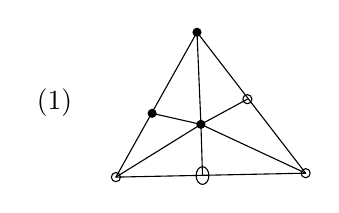
\begin{tikzpicture}[x=1cm,y=1cm,line cap=round,line join=round]
\coordinate (T) at (1.03,1.84);
\coordinate (L) at (0,0);
\coordinate (R) at (2.41,.05);
\coordinate (TL) at (.46,.81);
\coordinate (TR) at (1.67,.99);
\coordinate (B) at (1.1,.02);
\coordinate (C) at (1.08,.67);
\node[anchor=east] at (-.43,.95) {(1)};
\draw (L)--(T)--(R)--cycle;
\draw (T)--(C)--(B) (L)--(C)--(TR) (R)--(C)--(TL);
\foreach \point in {T,TL,C} \fill (\point) circle[radius=1.65pt];
\foreach \point in {L,R,TR} \draw (\point) circle[radius=1.65pt]; \draw (B) ellipse[x radius=2.3pt,y radius=3.2pt];
\end{tikzpicture}}\endgroup}\par\smallskip
Видно семь отмеченных точек и три внутренние линии. Нижняя средняя петля выступает под основание. Отдельной линии через три точки на сторонах не видно.}
\end{GelfandAdjacentEvidence}
\begin{GelfandAdjacentEvidence}{GELFAND-P001230}{8}

(конфигур. Фано)\qquad над \(\mathbb R,\mathbb Z\) не реализуется.

Верное предст. решётки \(=\) её отображение
\begin{equation*}
a:\Gamma\longrightarrow\mathcal L(F^n)\quad\text{--- реш. подпр-в,}
\end{equation*}
такое что
\begin{equation*}
\gamma_1<\gamma_2\ \Rightarrow\ a(\gamma_1)<a(\gamma_2)
\end{equation*}
и \(\sup\) сохраняется

(1) не реализуется [зачёркнуто] над \(\mathbb R\), но над \(\mathbb Z_2\) реализу..
\Unclear{GELFAND-P001230}{realization-cancel}{Знак перед «над» зачёркнут и не разобран.}
\end{GelfandAdjacentEvidence}



\Needspace{7\baselineskip}
\begin{GelfandAdjacentEvidence}{GELFAND-P001231}{1}
\SourcePage{GELFAND-P001231}{unlabelled}
Верное предст. есть у конфигур. (1):
\begin{equation*}
?\qquad m=4,\quad E,\quad \underline F,\quad \underline{\mathbb R^6}
\end{equation*}
\EvidenceBlock{GELFAND-P001231}{opening-symbols}{В строке с вопросительным знаком отдельно записаны \(m=4\), \(E\), \(F\) и \(\mathbb R^6\).}{Запись в рукописи.}
\end{GelfandAdjacentEvidence}
\begin{GelfandAdjacentEvidence}{GELFAND-P001231}{2}


Зад. о реализуемости \(\Leftrightarrow\) зад. о реш. системы алгебраических нер-в.
\EvidenceBlock{GELFAND-P001231}{inequalities-reading}{После «алгебраических» написано «нер-в.» (неравенств).}{Запись в рукописи.}
\end{GelfandAdjacentEvidence}
\begin{GelfandAdjacentEvidence}{GELFAND-P001231}{3}


\uwave{Нетрив. раб. по структурам:} (по Гельфанду)
\EvidenceBlock{GELFAND-P001231}{lattice-heading}{Первое сокращение в заголовке читается «Нетрив.».}{Запись в рукописи.}
\end{GelfandAdjacentEvidence}
\begin{GelfandAdjacentEvidence}{GELFAND-P001231}{4}


Дедекинд: придумал

Курош, Оре.

фон Нейман;

Гельфанд, Пономарёв:

[На левом поле: \uwave{Доб. Вершика:}]
\uwave{Пудлак и Тум} (Чехи): всякая конечная решётка вкладывается в решётку разбиений конечного мн-ва (очень трудная теорема).

(\(\inf\) и \(\sup\) --- [зачёркнуто] пересеч. и объед.)
\Incomplete{GELFAND-P001231}{inf-sup-cancel}{Слово после «inf и sup» зачёркнуто и не разобрано.}
\end{GelfandAdjacentEvidence}
\begin{GelfandAdjacentEvidence}{GELFAND-P001231}{5}


\(0\) --- разб. на точки.

\medskip
\underline{\underline{Фейгин Б.}}\qquad\underline{О струнах} [зачёркнуто] (продолжение).
\Unclear{GELFAND-P001231}{string-heading-cancel}{Вертикальный зачёркнутый знак после «О струнах» не разобран.}
\end{GelfandAdjacentEvidence}
\begin{GelfandAdjacentEvidence}{GELFAND-P001231}{6}


\underline{Операторная теория струн.}

\underline{Дуальные амплитуды.} Рассм. столкновение частиц

\SourceFigure{GELFAND-P001231}{scattering-diagram}{%
\par\smallskip
{\color{black}\begingroup\color{black}\GelfandFitDiagram{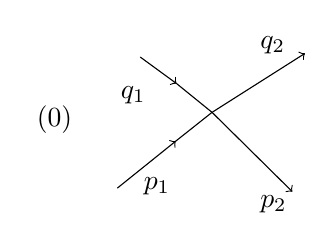
\begin{tikzpicture}[x=1cm,y=.96cm,line cap=round]
\node at (-2,0) {(0)};
\coordinate (lowerin) at (-1.2,-.90);
\coordinate (upperin) at (-.91,.83);
\coordinate (crossing) at (0,.10);
\coordinate (upperout) at (1.18,.88);
\coordinate (lowerout) at (1.02,-.95);
\draw[->] (lowerin)--(-.46,-.28);
\draw[->] (-.46,-.28)--(crossing)--(upperout);
\draw[->] (upperin)--(-.45,.48);
\draw[->] (-.45,.48)--(crossing)--(lowerout);
\node[below] at (-.70,-.63) {\(p_1\)};
\node[left] at (-.72,.33) {\(q_1\)};
\node[above] at (.77,.74) {\(q_2\)};
\node[below] at (.78,-.87) {\(p_2\)};
\end{tikzpicture}}\endgroup}\par\smallskip}
\end{GelfandAdjacentEvidence}
\begin{GelfandAdjacentEvidence}{GELFAND-P001231}{7}


Массы пусть все одинаковы и полный импульс \(=0\)

Всё --- векторы в пр-ве/времени
\begin{equation*}
\begin{cases}
p_1+q_1=p_2+q_2,\\
p_1^2=q_1^2=p_2^2=q_2^2=m^2
\end{cases}
\qquad p_j,q_j\in\mathbb R^4.
\tag{1}
\end{equation*}
\EvidenceBlock{GELFAND-P001231}{mass-shell-overwrite}{Переправленная буква с индексом в предпоследнем квадрате читается \(q_2\).}{Запись в рукописи.}
\end{GelfandAdjacentEvidence}
\begin{GelfandAdjacentEvidence}{GELFAND-P001231}{8}


Пусть дана \(S\)-матрица, характериз. это столкновение,
\begin{equation*}
S(p_1,q_1,p_2,q_2)\tag{2}
\end{equation*}
Переменные Мандельстама:
\begin{equation*}
\begin{cases}
s=(p_1+q_1)^2,\\
t=(p_1-p_2)^2\\
u\ \text{[зачёркнуто]}=(p_1-q_2)^2
\end{cases}\tag{3}
\end{equation*}
\Unclear{GELFAND-P001231}{mandelstam-u-cancel}{После \(u\) перед равенством зачёркнут неразобранный знак.}
\end{GelfandAdjacentEvidence}
\begin{GelfandAdjacentEvidence}{GELFAND-P001231}{9}

[Справа от (3):] (Заданы релятивистски инвариантные попарные скал. произведения)

зависимы:
\begin{equation*}
s+t+u=4m^2\tag{4}
\end{equation*}
Зададим \(A(s,t)\) (\(=\) выражение \(S\) через \(s,t\))

\uwave{Требование}:
\begin{equation*}
1)\quad A\text{ аналитична по }s,t\quad\text{[зачёркнуто]}\tag{5}
\end{equation*}
\Unclear{GELFAND-P001231}{analytic-tail}{После \(t\) зачёркнут знак. Его чтение не установлено.}
\end{GelfandAdjacentEvidence}



\Needspace{7\baselineskip}
\begin{GelfandAdjacentEvidence}{GELFAND-P001232}{1}
\SourcePage{GELFAND-P001232}{16}
2) \(A\) симметрична по \(s,t\) (независ. от порядка)

3) При фиксир. \(t\) ф-я \(A(s,t)\) имеет по \(s\) только простые полюса,
причём [вписано между словами: 4)] места полюсов не зависят от \(t\). Обычно пишут:
\begin{equation*}
A(s,t)=\sum_{n=0}^{\infty}\frac{R_n(t)}{n-\alpha(s)}\tag{6}
\end{equation*}
5) \(R_n(t)\) --- многочлен

График \(\alpha(s)\) наз. траекторией Редже.

Оказ., что из 1)---5) однозначно находим вид ф-и \(A\):
\begin{equation*}
A(s,t)=\frac{\Gamma(-\alpha(s))\Gamma(-\alpha(t))}{\Gamma(-\alpha(s)-\alpha(t))}
=B(-\alpha(s),-\alpha(t))\tag{7}
\end{equation*}
Из анализа экспер. данных вытекает, что
\begin{equation*}
\alpha(s)\quad\text{--- линейная ф-я}\tag{8}
\end{equation*}
\(A\) наз. амплитудой Венециано, или дуальной амплитудой, а усл. 1)---5) наз. \underline{условиями дуальности}.

Операторный метод: хотим записать \(A(s,t)\) как опер. среднее
\begin{equation*}
\langle0|V(t)V(s)|0\rangle,\tag{9}
\end{equation*}
где \(\langle0|\) --- вак. вектор в каком-то пр-ве, \(V(t)\) --- операторы.

Другая запись (7):
\begin{equation*}
S(p_1,p_2,p_3,p_4)=\int_0^1
x^{-2\langle p_1,p_2\rangle}(1-x)^{-2\langle p_2,p_3\rangle}
(x(1-x))^{-1-m^2}\,dx\tag{10}
\end{equation*}
Здесь

\SourceFigure{GELFAND-P001232}{amplitude-arrow-convention}{%
\par\smallskip
{\color{black}\begingroup\color{black}\GelfandFitDiagram{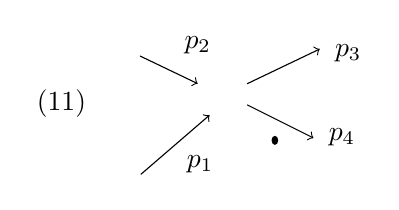
\begin{tikzpicture}[x=1cm,y=1cm,line cap=round]
\node at (-2.1,0) {(11)};
\draw[->] (-1.1,.60)--(-.37,.25);
\draw[->] (-1.09,-.90)--(-.22,-.15);
\draw[->] (.26,.25)--(1.18,.69);
\draw[->] (.26,-.02)--(1.1,-.44);
\node[above] at (-.37,.50) {\(p_2\)};
\node[below] at (-.34,-.54) {\(p_1\)};
\node[right] at (1.25,.64) {\(p_3\)};
\node[right] at (1.17,-.43) {\(p_4\)};
\fill (.61,-.47) ellipse[x radius=1.2pt,y radius=1.65pt];
\end{tikzpicture}}\endgroup}\par\smallskip
Рядом с нижней правой стрелкой виден чернильный след. Его связь со стрелкой неясна.}
\end{GelfandAdjacentEvidence}
\begin{GelfandAdjacentEvidence}{GELFAND-P001232}{2}

\begin{equation*}
p_1+p_2+p_3+p_4=0.
\end{equation*}
Аналогично можно писать амплитуды для большего числа частиц,
например:
\begin{equation*}
A(p_1,p_2,p_3,p_4,p_5)\cong\int\int_0^1
x^{\cdots}y^{\cdots}(1-x)^{\cdots}(1-y)^{\cdots}(1-xy)^{\cdots}\,dx\,dy\tag{12}
\end{equation*}
Эта амплитуда уже не вычислена в общем виде, только при нек-рых спец. значениях \underline{скал. произведений}.

Пр-во порождено конечным набором осцилляторов, к-рые соед. как в струне. Конечным числом обойтись нельзя!.
\EvidenceBlock{GELFAND-P001232}{finite-oscillators}{В первом предложении написано «конечным», во втором --- «Конечным числом обойтись нельзя!».}{Запись в рукописи.}
\end{GelfandAdjacentEvidence}
\begin{GelfandAdjacentEvidence}{GELFAND-P001232}{3}


Рассм. алгебру с образующими
\begin{equation*}
a_m^\mu,x^\mu,\quad \mu=0,1,\ldots,d,\quad
\text{[зачёркнуто]}\tag{13}
\end{equation*}
\Incomplete{GELFAND-P001232}{generators-cancel}{Запись после \(d\) в (13) зачёркнута и не разобрана.}
\end{GelfandAdjacentEvidence}

где \(d\) --- разм. пр-ва


\Needspace{7\baselineskip}
\begin{GelfandAdjacentEvidence}{GELFAND-P001233}{1}
\SourcePage{GELFAND-P001233}{unlabelled}
\begin{equation*}
\relax [a_m^\mu,a_n^\nu]=m g^{\mu\nu}\delta_{m,-n}\tag{14}
\end{equation*}
\(m,n\) --- целые числа
\begin{equation*}
a_0^\mu=p^\mu\tag{15}
\end{equation*}
\begin{equation*}
\relax [x^\mu,p^\nu]=i g^{\mu\nu}\tag{16}
\end{equation*}
\EvidenceBlock{GELFAND-P001233}{momentum-superscript}{Переправленный верхний индекс у \(p\) в (16) читается \(\nu\).}{Запись в рукописи.}
\end{GelfandAdjacentEvidence}
\begin{GelfandAdjacentEvidence}{GELFAND-P001233}{2}

\begin{equation*}
\relax [x^\mu,a_m^\nu]=0,\quad m\ne0\tag{17}
\end{equation*}
Смысл образующих \(x^\mu,a_m^\mu\):

[Зачёркнуто: \(p^\mu\) --- не разобрано]
\Unclear{GELFAND-P001233}{coordinates-cancel}{В начале зачёркнутой записи читается \(p^\mu\). Остальные знаки неразборчивы.}
\end{GelfandAdjacentEvidence}
\begin{GelfandAdjacentEvidence}{GELFAND-P001233}{3}

\((x^\mu,p^\mu)\) --- коорд. и импульс центра тяжести летящей струны, \(a_m^\mu\) --- разлож. в ряд Фурье всего остального.

Положим:
\begin{equation*}
P^\mu(\theta)=\sum_{-\infty}^{+\infty}a_m^\mu e^{-im\theta},\tag{18}
\end{equation*}
(импульс точки с парам. \(\theta\))
\begin{equation*}
Q^\mu(\theta)=x^\mu+a_0^\mu\theta+
 i\sum_{\substack{n=-\infty\\n\ne0}}^{\infty}\frac1n a_{[m?]}^\mu e^{-in\theta}.\tag{19}
\end{equation*}
\Unclear{GELFAND-P001233}{fourier-index}{Переправленный нижний индекс при \(a\) предположительно читается \(m\), возможно \(n\). В сумме и показателе экспоненты написано \(n\).}
\end{GelfandAdjacentEvidence}
\begin{GelfandAdjacentEvidence}{GELFAND-P001233}{4}

Тогда выполнены коммутационные соотношения:
\begin{equation*}
\relax [Q_\mu(\theta),P_\nu(\theta')]=2\pi i g_{\mu\nu}\delta(\theta-\theta')\tag{20}
\end{equation*}
\begin{equation*}
\relax [P_\mu(\theta),P_\nu(\theta')]=2\pi i g_{\mu\nu}\delta'(\theta-\theta')\tag{21}
\end{equation*}
\begin{equation*}
\relax [Q_\mu(\theta),Q_\nu(\theta')]=-\pi i g_{\mu\nu}\varepsilon(\theta-\theta'),\tag{22}
\end{equation*}
где \(\varepsilon\) --- ф-я Хевисайда
\Unclear{GELFAND-P001233}{heaviside-convention}{Написано «где \(\varepsilon\) --- ф-я Хевисайда». Нормировка здесь не указана.}
\end{GelfandAdjacentEvidence}
\begin{GelfandAdjacentEvidence}{GELFAND-P001233}{5}

\begin{equation*}
L_m\overset{\mathrm{def}}{=}\frac1{4\pi}\int_0^{2\pi}
e^{im\theta}:P^2(\theta):\,d\theta\tag{23}
\end{equation*}
Тогда получ. представление алгебры Вирасоро
\begin{equation*}
\relax [L_m,L_n]=(m-n)L_{m+n}+\frac d{12}(m^3-m)\delta_{m,-n}\tag{24}
\end{equation*}
\Unclear{GELFAND-P001233}{central-dimension}{Коэффициент центрального члена написан \(\frac{d}{12}\).}
\end{GelfandAdjacentEvidence}


\uwave{Упражнение}: проверить это.

Кстати,
\begin{equation*}
L_0=\frac12a_0^2+\sum_{n=1}^{\infty}a_{-n}a_n\tag{25}
\end{equation*}


\Needspace{7\baselineskip}
\begin{GelfandAdjacentEvidence}{GELFAND-P001234}{1}
\SourcePage{GELFAND-P001234}{17}
\begin{equation*}
2L_m={:}\sum_{r+s=m}a_ra_s{:}\tag{26}
\end{equation*}
\uwave{Вертексный оператор}: положим
\begin{equation*}
V(k,\theta)=\exp\langle ik,Q(\theta)\rangle,\tag{27}
\end{equation*}
где \(k\) --- вектор, тогда
\begin{equation*}
V(k)=V(k,0)=
\exp\left\langle k,\sum_{n=1}^{\infty}\frac{a_{-n}}n\right\rangle
\exp(ikx)
\exp\left\langle-k,\sum_{n=1}^{\infty}\frac{a_n}n\right\rangle
\tag{28}
\end{equation*}
\EvidenceBlock{GELFAND-P001234}{vertex-insertion}{Множитель \(\exp(ikx)\) вписан над строкой. Линии от вставки сходятся между двумя экспонентами.}{Запись в рукописи.}
\end{GelfandAdjacentEvidence}
\begin{GelfandAdjacentEvidence}{GELFAND-P001234}{2}

и
\begin{equation*}
V(k,\theta)=\exp(i\theta L_0)V(k)\exp(-i\theta L_0).\tag{29}
\end{equation*}
Далее,

[Зачёркнуто перед (30)]
\begin{equation*}
\relax [L_n-L_0,V(k)]=\frac{nk^2}2V(k).\tag{30}
\end{equation*}
\Incomplete{GELFAND-P001234}{commutator-cancel}{Запись перед коммутатором (30) зачёркнута и не разобрана.}
\end{GelfandAdjacentEvidence}
\begin{GelfandAdjacentEvidence}{GELFAND-P001234}{3}


Рассмотрим серию взаимодействий:

\SourceFigure{GELFAND-P001234}{interaction-chain}{%
\par\smallskip
{\color{black}\begingroup\color{black}\GelfandFitDiagram{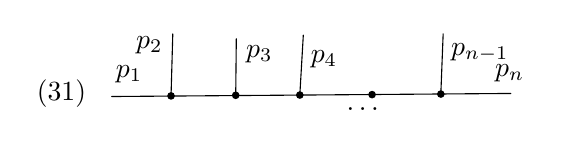
\begin{tikzpicture}[x=.74cm,y=.78cm,line cap=round]
\node at (-.86,.05) {(31)};
\draw (0,0)--(6.85,.05);
\draw (1.02,.01)--(1.05,1.02) (2.13,.02)--(2.14,.94)
      (3.23,.024)--(3.29,1.0) (5.65,.04)--(5.69,1.02);
\foreach \x/\y in {1.02/.01,2.13/.02,3.23/.024,4.47/.031,5.65/.04}
   \fill (\x,\y) circle[radius=1.38pt];
\node[above] at (.30,.06) {\(p_1\)};
\node[left] at (1.04,.83) {\(p_2\)};
\node[right] at (2.14,.69) {\(p_3\)};
\node[right] at (3.25,.61) {\(p_4\)};
\node[right] at (5.66,.72) {\(p_{n-1}\)};
\node[above] at (6.83,.08) {\(p_n\)};
\node[below] at (4.31,-.02) {\(\ldots\)};
\end{tikzpicture}}\endgroup}\par\smallskip}
\end{GelfandAdjacentEvidence}
\begin{GelfandAdjacentEvidence}{GELFAND-P001234}{4}


и по такой картинке построим амплитуду:
\begin{equation*}
\langle0|V(p_2)D(s_2)V(p_3)D(s_3)\ldots D(s_{n-2})V(p_{n-1})|0\rangle,
\tag{32}
\end{equation*}
\EvidenceBlock{GELFAND-P001234}{last-propagator-index}{Переправленная цифра в последнем аргументе \(D\) читается \(2\). Написано \(s_{n-2}\).}{Запись в рукописи.}
\end{GelfandAdjacentEvidence}

где \(p\) --- то же самое, что и \(k\),
\begin{equation*}
\begin{aligned}
s_2&=(p_2+p_1)^2\\
s_3&=(p_3+p_2+p_1)^2,\\
&\ldots
\end{aligned}\tag{33}
\end{equation*}
\begin{equation*}
D(s)=\int_0^1 x^{L_0-\alpha(s)-1}(1-x)^{\alpha(0)-1}\,dx,\tag{34}
\end{equation*}
где \(\alpha(s)\) --- линейная ф-я (траектория Редже).

(32) --- дуальная амплитуда; она должна совпадать с \(A\), когда 4 вершины.

Разложим \(V(k,\theta)\) в ряд Фурье:
\begin{equation*}
V(k,\theta)=\sum V_n(k)e^{-in\theta}.\tag{35}
\end{equation*}
Имеются операторы \(a_i^\mu\) и \(a_0^\mu\) и вакуумные векторы
\(|0,p\rangle\), удовлетв. условию


\Needspace{7\baselineskip}
\begin{GelfandAdjacentEvidence}{GELFAND-P001235}{1}
\SourcePage{GELFAND-P001235}{unlabelled}
\begin{equation*}
a_i^\mu|0,p\rangle=0,\quad\text{если }i>0,
\tag*{$(36)_i$}
\end{equation*}
\begin{equation*}
a_0^\mu|0,p\rangle=
\text{[зачёркнуто]}\ p^\mu\,\text{[зачёркнуто]}\ |0,p\rangle.
\tag*{$(36)_0$}
\end{equation*}
\Unclear{GELFAND-P001235}{vacuum-cancel-left}{зачёркнутая запись перед $p^\mu$}
\end{GelfandAdjacentEvidence}
\begin{GelfandAdjacentEvidence}{GELFAND-P001235}{2}

\Unclear{GELFAND-P001235}{vacuum-cancel-right}{зачёркнутый знак после $p^\mu$}
\end{GelfandAdjacentEvidence}
\begin{GelfandAdjacentEvidence}{GELFAND-P001235}{3}

(вакуумы занумерованы векторами импульса)

Получим пр-во
\begin{equation*}
\bigoplus_p H(p)
\tag{37}
\end{equation*}
Вертексный оператор действует так:
\begin{equation*}
V_n(k):H(p)\longrightarrow H(p+k).
\tag{38}
\end{equation*}
Коммутационные соотношения:

[Зачёркнуто: неразборчиво]
\Incomplete{GELFAND-P001235}{commutator-cancel}{Зачёркнутая запись под заголовком «Коммутационные соотношения» не прочитана.}
\end{GelfandAdjacentEvidence}
\begin{GelfandAdjacentEvidence}{GELFAND-P001235}{4}

\begin{equation*}
\relax [a_m^\mu,V_n(k)]=V_{n+m}(k)\cdot k_\mu
\tag{39}
\end{equation*}
\EvidenceBlock{GELFAND-P001235}{commutator-index}{В множителе \(k_\mu\) в (39) индекс \(\mu\) написан внизу.}{Запись в рукописи.}
\end{GelfandAdjacentEvidence}
\begin{GelfandAdjacentEvidence}{GELFAND-P001235}{5}


[Зачёркнуто: $V_n(k_1)|0,p\rangle$ / $V_1(k_1)|0,p\rangle$\textsuperscript{?}] Положим
\Unclear{GELFAND-P001235}{vertex-cancel}{В зачёркнутой записи читаются \(V\), \((k_1)\) и \(\lvert 0,p\rangle\). Нижний индекс \(V\) предположительно \(n\) или \(1\).}
\end{GelfandAdjacentEvidence}
\begin{GelfandAdjacentEvidence}{GELFAND-P001235}{6}

\begin{equation*}
\langle0,p+k_1+k|V_{-n}(k_2)V_n(k_1)|0,p\rangle=A_n\qquad\text{(это числа)}
\tag{40}
\end{equation*}
\EvidenceBlock{GELFAND-P001235}{bra-last-momentum}{В бра-векторе (40) написано \(p+k_1+k\). У последнего \(k\) нет нижнего индекса.}{Запись в рукописи.}
\end{GelfandAdjacentEvidence}


Тогда
\begin{equation*}
\sum A_n z^n=(1-z)^{\langle k_1,k_2\rangle}.
\tag{41}
\end{equation*}
Это доказывается простым вычислением. Предлагается проверить (41) в качестве упражнения.


\Needspace{7\baselineskip}
\begin{GelfandAdjacentEvidence}{GELFAND-P001236}{1}
\SourcePage{GELFAND-P001236}{26}
\underline{18/XI–85г.}\qquad \underline{Сем. Гельфанда}

\underline{Б. Фейгин} (продолжение).

$L_i$ — образующие алг. Вирасоро; пусть есть большое пр-во, в к-ром действ. эта алгебра

Соб. векторы $L_0=$ весовые векторы

$L_i$ действует в пр-ве весовых векторов из коммут. соотношений

(см. (24) на стр. 17 лев.)

Старший [зачёркнуто: вектор?\textsuperscript{?}] вес: вектор, к-рый нельзя уже повысить
\Unclear{GELFAND-P001236}{highest-cancel}{Зачёркнутое слово предположительно читается «вектор». Середина слова перекрыта штрихами.}
\end{GelfandAdjacentEvidence}
\begin{GelfandAdjacentEvidence}{GELFAND-P001236}{2}

\begin{equation*}
\widetilde{\mathcal H}=\{v\mid L_0v=v,\quad L_iv=0\ \text{при }i>0\}.\qquad\text{(вес 1)}
\tag{1}
\end{equation*}
\begin{equation*}
\overline{\mathcal H}=\{v\in\widetilde{\mathcal H},\quad v=L_i v',\ i<0\},
\tag{2}
\end{equation*}
[Справа:] здесь $v'$ — произв. весовой вектор из большого пр-ва.

(пр-во «спурионов» — назв. физиков, $\sim15$ лет назад)
\begin{equation*}
\mathcal H\overset{\mathrm{def}}{=}\widetilde{\mathcal H}/\overline{\mathcal H}
\tag{3}
\end{equation*}
\begin{equation*}
\prod_{i=1}^N a_{m_i}^{\mu_i}|0,p\rangle
\tag{4}
\end{equation*}
[Справа:] (пр-во состояний)

большой модуль над алг. Вирасоро
\begin{equation*}
L_{-1}v'=v\quad\Rightarrow\quad v'\text{ имеет вес }2:\quad L_0v'=2v'
\tag{5}
\end{equation*}
\EvidenceBlock{GELFAND-P001236}{weight-two}{В (5) написано \(L_{-1}v'=v\), «\(v'\) имеет вес 2» и \(L_0v'=2v'\).}{Запись в рукописи.}
\end{GelfandAdjacentEvidence}
\begin{GelfandAdjacentEvidence}{GELFAND-P001236}{3}


Цель: факторизация отн. группы диффеом. во всём пр-ве, но действует центр. расширение, и центр действ. нетривиально.

Предлаг. другая процедура получ. «инвар.» векторов: относит. половины они инвар., затем факторизуем по действию других и отбрасываем.

Алг. Вирасоро исчезает, от неё остаётся пр-во инвариантов.

Хотим:

I. Построить пр-во, порожд. $d-2$ осцилляторами.

II. Док., что все векторы в $\widetilde{\mathcal H}/\overline{\mathcal H}$ имеют норму $>0$

(в исх. $d$-мерном это не так)

(отсутствие \underline{тахионов\textsuperscript{?}})
\EvidenceBlock{GELFAND-P001236}{tachyon-word}{Подчёркнутое слово читается «тахионов».}{Запись в рукописи.}
\end{GelfandAdjacentEvidence}


В размерности 26 это всё достигается.


\Needspace{7\baselineskip}
\begin{GelfandAdjacentEvidence}{GELFAND-P001237}{1}
\SourcePage{GELFAND-P001237}{unlabelled}
Вертексные операторы:
\begin{equation*}
X(p,z)=\exp\left(p_\mu\cdot\sum_{n=1}^{\infty}a_{-n}^\mu z^n\right)D_p
\exp\left(-p_\mu\sum_{n=1}^{\infty}\frac{a_n^\mu}{n}z^{-n}\right),
\tag{6}
\end{equation*}
\EvidenceBlock{GELFAND-P001237}{left-exponential-normalization}{В левой экспоненте (6) написано \(a_{-n}^{\mu}z^n\) без дробной черты и знаменателя.}{Запись в рукописи.}
\end{GelfandAdjacentEvidence}
\begin{GelfandAdjacentEvidence}{GELFAND-P001237}{2}


где операторы $D_p$ опред. ф-лами
\begin{equation*}
D_p|0,k\rangle=|0,k+p\rangle,\quad [D_p,a_n^\mu]=0,\ n\ne0.
\tag{7}
\end{equation*}
Корреляционная функция:
\begin{equation*}
\begin{aligned}
&\langle0,k+\textstyle\sum p_i|X(z_1,p_1)\ldots X(z_n,p_n)|0,k\rangle\\
&\qquad=\prod_{j>1}\left(1-\frac{z_j}{z_i}\right)^{\langle p_i,p_j\rangle}.
\end{aligned}
\tag{8}
\end{equation*}
\EvidenceBlock{GELFAND-P001237}{product-index}{Под знаком произведения написано \(j>1\). Последний знак имеет нижнюю ножку цифры \(1\).}{Запись в рукописи.}
\end{GelfandAdjacentEvidence}
\begin{GelfandAdjacentEvidence}{GELFAND-P001237}{3}


Разлагая $X(z,p)$ в ряд, получим:
\begin{equation*}
X(z,p)=\sum X_i(p)z^i
\tag{9}
\end{equation*}
(это определение операторов $X_i(p)$)

Хотим построить 24 осциллятора.

Далее будут строиться операторы
\begin{equation*}
\int X(p,z)\frac{dz}{z},
\tag{10}
\end{equation*}
коммутирующие с алг. Вирасоро при $\langle p,p\rangle=2$.
\begin{equation*}
\begin{aligned}
&\text{На }\mathbb R^{26}\text{ хотим иметь }p_1,\ldots,p_n:\quad\langle p_i,p_i\rangle=2\\
&\langle p_i,p_j\rangle=A_{ij}\in\mathbb Z,\quad A_{ij}<0.
\end{aligned}
\tag{11}
\end{equation*}
[На левом поле: зачёркнутый вертикальный знак\textsuperscript{?}]
\Unclear{GELFAND-P001237}{cartan-margin-cancel}{зачёркнутый вертикальный знак}
\end{GelfandAdjacentEvidence}
\begin{GelfandAdjacentEvidence}{GELFAND-P001237}{4}


\EvidenceBlock{GELFAND-P001237}{cartan-diagonal}{Написано \(A_{ij}<0\). Рядом с неравенством нет ограничения на индексы.}{Запись в рукописи.}
\end{GelfandAdjacentEvidence}


Тогда операторы
\begin{equation*}
e_i=\int X(p_i,z)\frac{dz}{z},\quad f_i=\int X(-p_i,z)\frac{dz}{z}
\tag{12}
\end{equation*}
порождают на пр-ве действие алгебры Каца–Муди с матрицей Картана $A_{ij}$; при этом надо ещё положить
\begin{equation*}
h_i|0,k\rangle=\langle k,p_i\rangle|0,k\rangle
\tag{13}
\end{equation*}
\underline{Читать}: \underline{ст. МакДональда} (начало), \underline{Sem. Bourbaki};

учить алгебры Ли по ней.

[На левом поле: И.М.Г.] В самой большой простой конечной группе $\sim10^{54}$ элементов; она связана со струнами!

[Приписано справа:] (монстр «Лунное сияние»)

Moonshine

(есть раб. Френкель, Леповский и кто-то ещё)

Как-то получ. фунд. предст. алг. Каца–Муди.


\Needspace{7\baselineskip}
\begin{GelfandAdjacentEvidence}{GELFAND-P001238}{1}
\SourcePage{GELFAND-P001238}{27}
В $\mathbb R^{26}$ рассмотрим метрику $\langle-1,1,1,\ldots,1\rangle$,

[Зачёркнуто: нулев…?] вектор длины 0, [зачёркнуто: неразборчиво]
\Unclear{GELFAND-P001238}{null-cancel-before}{Зачёркнутая запись предположительно читается «нулев…». Конец слова неразборчив.}
\end{GelfandAdjacentEvidence}
\begin{GelfandAdjacentEvidence}{GELFAND-P001238}{2}

\Incomplete{GELFAND-P001238}{null-cancel-after}{Зачёркнутое слово после «вектор длины 0» не прочитано.}
\end{GelfandAdjacentEvidence}
\begin{GelfandAdjacentEvidence}{GELFAND-P001238}{3}


[Перед следующей строкой: две вертикальные отметки; правая похожа на фигурную скобку\textsuperscript{?}] 24 осциллятора
\Unclear{GELFAND-P001238}{null-marks}{Две разнесённые вертикальные отметки. Правая похожа на фигурную скобку с нижним крючком. Назначение отметок неясно.}
\end{GelfandAdjacentEvidence}
\begin{GelfandAdjacentEvidence}{GELFAND-P001238}{4}


(Обзор D. (?) Шварца 1973 года).
\Unclear{GELFAND-P001238}{schwarz-initial}{Перед «Шварца» виден округлый знак, предположительно D., рядом с вертикальными чертами. Инициал остаётся неясным.}
\end{GelfandAdjacentEvidence}


\begin{center}—\quad .\quad —\end{center}

$\mathbb R^d$ с индефин. метрикой и пусть дан вектор $p$ с $\langle p,p\rangle=0$

[Под «метрикой»:] (Минковского; 1 минус)

Положим
\begin{equation*}
U_n(v)=\int v(z)X(np,z)\frac{dz}{z},
\tag{14}
\end{equation*}
где $v\in\mathbb R^d$, $v=\sum v_i e_i$, $v(z)=\sum v_\mu a_n^\mu z^n$

Пусть
\begin{equation*}
v^1,v^2,\ldots,v^{d-2}\text{ — такие, что }\langle v^i,p\rangle=0
\tag{15}
\end{equation*}
\begin{GelfandAdjacentEvidence}{GELFAND-P001238}{5}
[Над зачёркнутым знаком вставлено «и»:] и [зачёркнуто: зачёркнутый знак под вставленным «и»\textsuperscript{?}]
\Unclear{GELFAND-P001238}{basis-cancel-left}{Над зачёркнутым знаком вписано «и». Зачёркнутый знак не разобран.}
\end{GelfandAdjacentEvidence}
\begin{GelfandAdjacentEvidence}{GELFAND-P001238}{6}

$v^1,v^2,\ldots,v^{d-2},p$ — базис в пр-ве
[зачёркнуто: неразборчиво] $\{x:\langle x,p\rangle=0\}$.
\Unclear{GELFAND-P001238}{basis-cancel-right}{Зачёркнутое слово после «в пр-ве», возможно, начинается с «в». Остальные буквы неразборчивы.}
\end{GelfandAdjacentEvidence}
\begin{GelfandAdjacentEvidence}{GELFAND-P001238}{7}


Положим
\begin{equation*}
b_n^\mu=U_n(v^\mu);
\tag{16}
\end{equation*}
$b_n^\mu$ образуют алг. Гейзенберга $\Rightarrow$ осцилляторы.

Они порождают всё пр-во.

Есть ещё обзор Грина и Шварца (томик Physics Reports).

\bigskip
\underline{Зелевинский А.}\qquad \underline{Клетки}
[над строкой вставлено: \underline{(и многочлены)}]
\underline{Шуберта и когомологии мн-зий флагов.}

О работах \underline{A. [зачёркнуто: неразборчивая помета] Lascoux}, \underline{M.-P. Schützenberger}
\Unclear{GELFAND-P001238}{lascoux-cancel}{Между «A.» и «Lascoux» зачёркнута помета, возможно буква или инициал. Она неразборчива.}
\end{GelfandAdjacentEvidence}
\begin{GelfandAdjacentEvidence}{GELFAND-P001238}{8}


(клетки Шуберта и когом. грассм. мн-зий; мн-зий флагов)

продолж. раб. Берншт., И.М.Г. и С.И.Г. УМН, 1973, 28:3, 3–26.

$X$ — мн-зие полных флагов в $V^n$ (флаги подпр-в)

[Под $X$, над (1): $\Vert$ (?), две вертикальные черты]
\Unclear{GELFAND-P001238}{flag-relation}{Под \(X\) две вертикальные черты, предположительно \(\Vert\). Между ними тонкий поперечный след на уровне линейки листа. Назначение знака неясно.}
\end{GelfandAdjacentEvidence}

\begin{equation*}
\{V^1\subset V^2\subset\ldots\subset V^n\}
\tag{1}
\end{equation*}
Когомологии опис. 2-мя способами

$1^{\circ}.$ \underline{Borel}
\begin{equation*}
H^*(X,\mathbb Q)=\mathbb Q[x_1,\ldots,x_n]/J
\end{equation*}
Идеал $J$ порождён симметр. многочленами без своб. члена

\Needspace{3\baselineskip}
$2^{\circ}.$ Базис в гомологиях $H_*(X,\mathbb Q)$ сост. клетки Шуберта $(c_w)$
\nopagebreak[4]
$w$ — перестановка чисел от 1 до $n$


\Needspace{7\baselineskip}
\begin{GelfandAdjacentEvidence}{GELFAND-P001239}{1}
\SourcePage{GELFAND-P001239}{unlabelled}
\begin{equation*}
\begin{array}{cccc}
1&2&\ldots&n\\
i_1&i_2&\ldots&i_n
\end{array}
\end{equation*}
Рассм. фикс. полный флаг
\begin{equation*}
F=(\langle e_1\rangle,\ \langle e_1,e_2\rangle,\ \langle e_1,e_2,e_3\rangle,\ldots,\ \langle e_1,e_2,\ldots,e_n\rangle).
\end{equation*}
Подействуем на него перест. $w$:
\begin{equation*}
F_w=(\langle e_{w(1)}\rangle,\ \langle e_{w(1)},e_{w(2)}\rangle,\ldots)
=(\langle e_{i_1}\rangle,\ \langle e_{i_1},e_{i_2}\rangle,\ldots).
\end{equation*}
[Зачёркнуто: [Клетка?]. Над зачёркнутым вставлено: $(C_w)\overset{\mathrm{def}}{=}$.]
\Unclear{GELFAND-P001239}{cancel-cell}{Начальный штрих похож на «К». Зачёркнутое слово предположительно читается «Клетка». Остальные буквы неразборчивы.}
\end{GelfandAdjacentEvidence}
\begin{GelfandAdjacentEvidence}{GELFAND-P001239}{2}

[Подчёркнуто: (Траектория флага $F_w$ под действием лин. преобразований, сохраняющих флаг $F$).]
[Зачёркнуто: неразборчивое обозначение.]
\Unclear{GELFAND-P001239}{cancel-after-orbit}{неразборчивое обозначение}
\end{GelfandAdjacentEvidence}
\begin{GelfandAdjacentEvidence}{GELFAND-P001239}{3}

\begin{equation*}
\dim_{\mathbb C} c_w=\ell(w)\text{ — число инверсий в }w.
\end{equation*}
Двойств. базис в когомологиях:
\begin{equation*}
P_w\in H^{2\ell(w)}(X;\mathbb Q).
\end{equation*}
Б.-Г.-Г. нашли явные ф-лы для $P_w$ в реализ. Бореля — многочлены (!).
[Под первым словом «многочлены»: $(\operatorname{mod}J)$.]
[Зачёркнуто: неразборчиво.]
\Unclear{GELFAND-P001239}{middle-cancel}{неразборчиво}
\end{GelfandAdjacentEvidence}
\begin{GelfandAdjacentEvidence}{GELFAND-P001239}{4}

Теперь их подняли и получились просто многочлены: их степени
\begin{equation*}
\operatorname{deg} P_w=\ell(w).
\end{equation*}
\begin{equation*}
P_{\mathrm{id}}=1.
\end{equation*}
\begin{equation*}
w_0=(n,n-1,\ldots,1).
\end{equation*}
Тогда
\begin{equation*}
\operatorname{deg} P_{w_0}=\frac{n(n-1)}{2}.
\end{equation*}
Неоднозначно выб., выберем
\begin{equation*}
P_{w_0}=x_1^{n-1}x_2^{n-2}\ldots x_{n-1}.
\end{equation*}
(У Б.-Г.-Г.: $\displaystyle\prod_{i<j}(x_i-x_j)$ — то же самое $\operatorname{mod}$ идеала.)
\EvidenceBlock{GELFAND-P001239}{bgg-normalization}{Перед произведением по \(i<j\) нет нормирующего множителя.}{Запись в рукописи.}
\end{GelfandAdjacentEvidence}
\begin{GelfandAdjacentEvidence}{GELFAND-P001239}{5}


Или: $\displaystyle\frac{\rho^{m(n-1)/2}}{\left(\frac{m(n-1)}{2}\right)!}$, где $\rho=(n-1)x_1+(n-2)x_2+\ldots$
\EvidenceBlock{GELFAND-P001239}{rho-degree}{И в показателе степени при \(\rho\), и под чертой перед скобкой \((n-1)\) написано \(m\).}{Запись в рукописи.}
\end{GelfandAdjacentEvidence}


Остальные выражаются:
\begin{equation*}
P_w=A_{w_0w^{-1}}P_{w_0},
\end{equation*}


\Needspace{7\baselineskip}
\begin{GelfandAdjacentEvidence}{GELFAND-P001240}{1}
\SourcePage{GELFAND-P001240}{28}
$A_w$ — опер., отвеч. перест.
\begin{equation*}
w=(i_1,i_1+1)(i_2,i_2+1)\ldots(i_{\ell(w)},i_{\ell(w)+1})
\end{equation*}
(произв. инверсий).
\EvidenceBlock{GELFAND-P001240}{top-last-index}{Во втором индексе последней транспозиции \(+1\) написано на уровне \(\ell(w)\), так что получается \(i_{\ell(w)+1}\).}{Запись в рукописи.}
\end{GelfandAdjacentEvidence}
\begin{GelfandAdjacentEvidence}{GELFAND-P001240}{2}


\begin{equation*}
A_{(i,i+1)}=
\frac{p(x_1,\ldots,x_i,x_{i+1},\ldots,x_n)-p(x_1,\ldots,x_{i+1},x_i,\ldots,x_n)}{x_{i+1}-x_i}.
\end{equation*}
[После знака равенства, перед дробью, зачёркнуто: $p(x_1,\ldots$; далее неразборчиво.]
\Unclear{GELFAND-P001240}{cancel-polynomial}{В зачёркнутой записи читается начало \(p(x_1,\ldots\). Далее виден знак, похожий на \(x\). Конечные индексы и скобки неразборчивы.}
\end{GelfandAdjacentEvidence}
\begin{GelfandAdjacentEvidence}{GELFAND-P001240}{3}

\EvidenceBlock{GELFAND-P001240}{fraction-sign}{В знаменателе написано \(x_{i+1}-x_i\).}{Запись в рукописи.}
\end{GelfandAdjacentEvidence}
\begin{GelfandAdjacentEvidence}{GELFAND-P001240}{4}


Оператор
\begin{equation*}
A_w=A_{(i_1,i_1+1)}\ldots A_{(i_{\ell(w)},i_{\ell(w)+1})}
\end{equation*}
\EvidenceBlock{GELFAND-P001240}{operator-last-index}{Во втором индексе последнего множителя \(+1\) написано на уровне \(\ell(w)\).}{Запись в рукописи.}
\end{GelfandAdjacentEvidence}


опред. корректно (не зав. от разложения в произведение инверсий).
Он и использован в ф-ле.

\underline{Усл. симметрии}.

$P_w$ симметричен отн. $x_i,x_{i+1}$, если $(i,i+1)$ не явл. инверсией для $w$.


\Needspace{7\baselineskip}
\begin{GelfandAdjacentEvidence}{GELFAND-P001241}{1}
\SourcePage{GELFAND-P001241}{35}
\underline{25/XI-85 г.}\qquad \underline{Сем. Гельфанда.}

\underline{Фейгин} (продолжение). (О струнах).

Образующие алгебры Вирасоро:
\begin{equation*}
L_i=:\sum_{m+n=i}g_{\mu\nu}a_m^\mu a_n^\nu:\tag{1}
\end{equation*}
\EvidenceBlock{GELFAND-P001241}{normal-order-normalization}{За открывающим двоеточием сразу следует знак суммы с условием \(m+n=i\).}{Запись в рукописи.}
\end{GelfandAdjacentEvidence}
\begin{GelfandAdjacentEvidence}{GELFAND-P001241}{2}


$:\quad:$ обеспечивают корректность опред. оператора и дают только добавление постоянной.

\underline{И.М.Г.} Что нужно, чтобы была операция $:\quad:$? Здесь она приводит к появлению алг. Вирасоро. Что если взять решетку или тор? Что на сфере?
\begin{equation*}
\relax [L_i,L_j]=(i-j)L_{i+j}+\delta_{i,-j}\frac{i^3-i}{12}\,c\tag{2}
\end{equation*}
\begin{equation*}
p^\mu(t)=\sum a_m^\mu e^{-imt},\qquad
q^\mu(t)=\sum_{m\ne0}\frac{a_m^\mu}{m}e^{-imt}+q_0^\mu\tag{3}
\end{equation*}
\begin{align*}
[x^\mu,a_m^\nu]&=0,\quad m\ne0,\\[0pt]
[x^\mu,a_0^\nu]&=g^{\mu\nu},\\
x^\mu(t)&=x^\mu+\sum_{n\ne0}\frac1n\bigl(a_n^\mu e^{-int}\bigr).
\end{align*}
\underline{И.М.Г.} В классич. теории:
\begin{equation*}
L_n=e^{int}\frac{d}{dt}.
\end{equation*}
Квант. механика соотв. одномерному расширению классич. теории: ср. $[\frac{d}{dx},x]=1$.

(4) $\mathcal H_p$ — модуль, порожденный высш. вектором $|p\rangle$.

[Справа: ([зачёркнуто] $a_m^\mu$ и тд). Над зачёркнутым вставлено «(примен.)», проведена линия к месту вставки.]
\Unclear{GELFAND-P001241}{module-margin}{Зачёркнутое обозначение перед \(a_m^\mu\) неразборчиво. С зачёркнутым местом соединена вставка «(примен.)».}
\end{GelfandAdjacentEvidence}
\begin{GelfandAdjacentEvidence}{GELFAND-P001241}{3}


[Между строками:] Это модуль над алг. Вирасоро.

(5) Структура его [зачёркнуто] зависит только от $\langle p,\ [\text{неразб.}]\ p\rangle$; по определению
\Unclear{GELFAND-P001241}{depends-cancel}{малый зачёркнутый знак перед «зависит»}
\end{GelfandAdjacentEvidence}
\begin{GelfandAdjacentEvidence}{GELFAND-P001241}{4}

\Unclear{GELFAND-P001241}{module-norm}{Переправленный знак между запятой и вторым \(p\) похож на \(\xi\). Его чтение и статус неясны.}
\end{GelfandAdjacentEvidence}


\begin{equation*}
a_m^\nu|p\rangle=0,\quad m>0,\qquad
 a_0^\nu|p\rangle=p^\nu|p\rangle\tag{6}
\end{equation*}
(5) $\mathcal H_p\cong\mathcal H_{p'}$, если $\langle p,p\rangle=\langle p',p'\rangle$.
$\Vert$ Обозначим его $\mathcal H_{\langle p,p\rangle}$.

Рассмотрим
\begin{equation*}
\bigoplus_{\langle p,p\rangle\in\mathbb R}\mathcal H_{\langle p,p\rangle}\tag{7}
\end{equation*}


\Needspace{7\baselineskip}
\begin{GelfandAdjacentEvidence}{GELFAND-P001242}{1}
\SourcePage{GELFAND-P001242}{unlabelled}
Определим из [зачёркнуто] модуля (7) пр-во физических состояний, как делалось [зачёркнуто] выше (стр. (26)).
\Unclear{GELFAND-P001242}{cancel-before-module}{неразборчивый зачёркнутый знак перед «модуля»}
\end{GelfandAdjacentEvidence}
\begin{GelfandAdjacentEvidence}{GELFAND-P001242}{2}

\Unclear{GELFAND-P001242}{cancel-before-above}{неразборчивый зачёркнутый знак перед «выше»}
\end{GelfandAdjacentEvidence}
\begin{GelfandAdjacentEvidence}{GELFAND-P001242}{3}


Конструкция зависит [над строкой вставлено: только] от [зачёркнуто] действия алг. Вирасоро.
\Unclear{GELFAND-P001242}{cancel-before-action}{Перед «действия» зачёркнуто слово, предположительно «определения». Середина неразборчива.}
\end{GelfandAdjacentEvidence}
\begin{GelfandAdjacentEvidence}{GELFAND-P001242}{4}


(8) \underline{Теорема}. (о духах).

1) Сущ. система осцилляторов $b_m^\mu$, $m\ne0$, $\mu=1,2,\ldots,24$
со станд. коммут. соотн. [неразобранный знак] на пр-ве [зачёркнуто; над строкой вставлено: физ. состояний] и такая, что
\Unclear{GELFAND-P001242}{oscillator-prefix}{Отдельный высокий петлеобразный знак предположительно читается как «д». Раскрытие неясно.}
\end{GelfandAdjacentEvidence}
\begin{GelfandAdjacentEvidence}{GELFAND-P001242}{5}

\Unclear{GELFAND-P001242}{cancel-physical-space}{неразборчивое зачёркнутое обозначение под вставкой «физ. состояний»}
\end{GelfandAdjacentEvidence}
\begin{GelfandAdjacentEvidence}{GELFAND-P001242}{6}

\begin{equation*}
\relax [L_i,b_m^\mu]=0.
\end{equation*}
$b_m^\mu$ можно постр. из $a$.

2) $\exists$ в пр-ве физ. сост. [сверху вставлено: $\widetilde{\mathcal H}$] вак. вектор $|0\rangle$,
и $\widetilde{\mathcal H}$ порождается векторами $|0\rangle$ и опер. $b_n^\nu$.
Это только при \underline{\underline{$d=26$}}.

3) В $\widetilde{\mathcal H}$ имеется естеств. квадр. форма, наследуемая с пр-ва (7), и она на $\widetilde{\mathcal H}$ положит. определена.
\begin{equation*}
X(p,z)=\exp\left(p_\mu\sum_{n=1}^{\infty}\frac{a_{-n}^\mu}{n}z^n\right)
D_p\exp\left(-p_\mu\sum_{n=1}^{\infty}\frac{a_n^\mu}{n}z^{-n}\right),\tag{9}
\end{equation*}
Здесь $D_p$ опред. формулой
\begin{equation*}
D_p|k\rangle=|k+p\rangle,\tag{10}
\end{equation*}
[Зачёркнуто: а при этом.] Причём
\begin{equation*}
\relax [D_p,a_n^\mu]=0,\quad n\ne0.\tag{11}
\end{equation*}
Коммутац. соотношения $X(p,z)$ и $a_n^\mu$: если
\begin{equation*}
X(p,z)=\sum X_j(p)z^j,
\end{equation*}
то
\begin{equation*}
\relax [a_n^\mu,X_i(p)]=p^\mu X_{i+n}(p).\tag{12}
\end{equation*}
\EvidenceBlock{GELFAND-P001242}{mode-convention}{В разложении написано \(z^j\), в правой части (12) написано \(X_{i+n}(p)\).}{Запись в рукописи.}
\end{GelfandAdjacentEvidence}
\begin{GelfandAdjacentEvidence}{GELFAND-P001242}{7}


\underline{Представление алгебры токов.}

Пр-во разм. $d$, рассм. в $\mathbb R^d$ решётку $Q$ (дискр. подгруппу), счит., что $Q$ целочисленна и унимодулярна: есть такой базис
\begin{equation*}
e_1,\ldots,e_d,\quad\text{что }\langle e_i,e_j\rangle\text{ целочисл. и }\det\langle e_i,e_j\rangle=1.\tag{13}
\end{equation*}
Чётная решётка:
\begin{equation*}
\forall\gamma\in Q:\quad\langle\gamma,\gamma\rangle\text{ — чётное}.\tag{14}
\end{equation*}

[Узкая полоса соседнего листа у правой границы кадра:] 
\Unclear{GELFAND-P001242}{right-edge}{Сверху вниз видны обрезанные «(», «(», «(», «(», короткий вертикальный штрих и «(»; содержимое скобок за границей кадра.}
\end{GelfandAdjacentEvidence}



\Needspace{7\baselineskip}
\begin{GelfandAdjacentEvidence}{GELFAND-P001243}{1}
\SourcePage{GELFAND-P001243}{36}
(15) \underline{Корень решётки}: такой вектор $\gamma\in Q$, что $\langle\gamma,\gamma\rangle=2$.

(16) [Зачёркнуто] Такие бывают начиная с размерности [зачёркнуто] $8$ [зачёркнуто], точнее,
[зачёркнуто] только в размерности, делящейся на $8$.
\Unclear{GELFAND-P001243}{cancel-before-these}{неразборчивая зачёркнутая отметка после (16)}
\end{GelfandAdjacentEvidence}
\begin{GelfandAdjacentEvidence}{GELFAND-P001243}{2}

\Unclear{GELFAND-P001243}{cancel-before-eight}{неразборчивый зачёркнутый знак перед $8$}
\end{GelfandAdjacentEvidence}
\begin{GelfandAdjacentEvidence}{GELFAND-P001243}{3}

\Unclear{GELFAND-P001243}{cancel-after-eight}{неразборчивый зачёркнутый знак после $8$}
\end{GelfandAdjacentEvidence}
\begin{GelfandAdjacentEvidence}{GELFAND-P001243}{4}

\Unclear{GELFAND-P001243}{cancel-before-only}{неразборчивый зачёркнутый знак перед «только»}
\end{GelfandAdjacentEvidence}
\begin{GelfandAdjacentEvidence}{GELFAND-P001243}{5}


\underline{Упражнение:} построить \underline{такую} решётку в $\mathbb R^8$.

\begin{center}—\quad .\quad —\end{center}

$Q$ — решётка (пока не обязательно чётная).

\underline{Кстати:} [Зачёркнуто] Решётки корней групп серии $A,D,E$ облад. этим св-вом (14).
\Unclear{GELFAND-P001243}{aside-cancel}{зачёркнутый знак перед «решётки»}
\end{GelfandAdjacentEvidence}
\begin{GelfandAdjacentEvidence}{GELFAND-P001243}{6}


Рассм. функцию:
\begin{equation*}
\varepsilon:Q\times Q\longrightarrow\{\pm1\}\tag{17}
\end{equation*}
\begin{equation*}
\varepsilon(\alpha,\beta)\cdot\varepsilon(\beta,\alpha)=(-1)^{\langle\alpha,\beta\rangle},
\qquad\alpha,\beta\in Q;\tag{18}
\end{equation*}
\EvidenceBlock{GELFAND-P001243}{epsilon-parity}{После равенства в (18) написано \(\alpha,\beta\in Q\).}{Запись в рукописи.}
\end{GelfandAdjacentEvidence}
\begin{GelfandAdjacentEvidence}{GELFAND-P001243}{7}

\begin{equation*}
\varepsilon(\alpha,\alpha)=-1\quad\text{если }\langle\alpha,\alpha\rangle=2.\tag{19}
\end{equation*}
$\Delta$ — мн-во корней решётки $Q$, т.е.
$\Delta=\{\gamma\in Q\mid\langle\gamma,\gamma\rangle=2\}$.

Пусть квадр. форма $\langle\ ,\ \rangle$ полож. определена.
Введём алгебру Ли:
\begin{equation*}
\mathfrak g=f+\sum_{\alpha\in\Delta}\mathbb Cx_\alpha,\tag{20}
\end{equation*}
где $f=\mathbb R^d\otimes\mathbb C=\mathbb C^d$.
\Unclear{GELFAND-P001243}{cartan-symbol}{Оба петлеобразных знака по начертанию читаются как \(f\). Какой символ имелся в виду, неясно.}
\end{GelfandAdjacentEvidence}
\begin{GelfandAdjacentEvidence}{GELFAND-P001243}{8}


Зададим структуру алг. Ли на $\mathfrak g$ по формулам:
\begin{equation*}
\relax [h,x_\alpha]=\langle h,\alpha\rangle x_\alpha;\tag*{$(21)_1$}
\end{equation*}
\begin{equation*}
\relax [x_\alpha,x_\beta]=0\quad\text{если }\alpha+\beta\notin\Delta\cup\{0\};\tag*{$(21)_2$}
\end{equation*}
\begin{equation*}
\relax [x_\alpha,x_\beta]=\varepsilon(\alpha,\beta)x_{\alpha+\beta}
\quad\text{если }\alpha+\beta\in\Delta;\tag*{$(21)_3$}
\end{equation*}
\begin{equation*}
\relax [x_\alpha,x_{-\alpha}]=-\alpha.\tag*{$(21)_4$}
\end{equation*}
Это важная конструкция конечномерных простых алгебр.
\EvidenceBlock{GELFAND-P001243}{construction-adjective}{Написано «важная».}{Запись в рукописи.}
\end{GelfandAdjacentEvidence}


Пусть теперь в конструкции, опис. выше, $p\in Q$,
$|p\rangle$ — вак. вектор, $\gamma\in\Delta$.
Рассмотрим вертексный оператор
\begin{equation*}
X^\varepsilon(\gamma,z)=X(\gamma,z)\cdot\varepsilon_\gamma;\tag*{$(22)_1$}
\end{equation*}
где
\begin{equation*}
\varepsilon_\gamma|p\rangle=\varepsilon(\gamma,p)|p\rangle,\tag*{$(22)_2$}
\end{equation*}


\Needspace{7\baselineskip}
\begin{GelfandAdjacentEvidence}{GELFAND-P001244}{1}
\SourcePage{GELFAND-P001244}{unlabelled}
\begin{equation*}
\relax [\varepsilon_\gamma,a_m^\mu]=0,\quad m\ne0.\tag*{$(22)_3$}
\end{equation*}
Теперь введём
\begin{equation*}
X^\varepsilon(\gamma,z)=\sum X_i^\varepsilon(\gamma)z^i.\tag{23}
\end{equation*}
В $\mathbb R^{24}$ есть спец. решетка (особая), к-рая встреч. здесь и в теории конечных простых групп.
Всего спорадических простых групп $26$.

(24) $\{X_n^\varepsilon(\gamma),a_n^\mu\}$ порождают [над строкой вставлено: проективное] предст. алг. токов на окружности.
\begin{equation*}
\relax [X_n^\varepsilon(\gamma_1),X_m^\varepsilon(\gamma_2)]=0,
\quad\text{если }\langle\gamma_1,\gamma_2\rangle>0\tag*{$(25)_1$}
\end{equation*}
\begin{equation*}
\begin{aligned}
&[X_n^\varepsilon(\gamma_1),X_m^\varepsilon(\gamma_2)]
=\varepsilon(\gamma_1,\gamma_2)X_{n+m}^\varepsilon(\gamma_1+\gamma_2),\\
&\qquad\text{если }\langle\gamma_1,\gamma_2\rangle=-1
\end{aligned}
\tag*{$(25)_2$}
\end{equation*}
и другие [зачёркнуто] соотн. пишутся.
\Unclear{GELFAND-P001244}{cancel-other-relations}{Зачёркнутое сокращение перед «соотн.» предположительно читается «подоб.».}
\end{GelfandAdjacentEvidence}
\begin{GelfandAdjacentEvidence}{GELFAND-P001244}{2}


В $\mathbb R^{26}$ выберем вектор $c$, такой что $\langle c,c\rangle=0$, и рассмотрим интегралы
\begin{equation*}
\int a(z)X(nc,z)\frac{dz}{z}\tag{26}
\end{equation*}
[У $a(z)$ зачёркнут верхний индекс.]
\Unclear{GELFAND-P001244}{cancel-integrand-index}{возможно, $\mu$}
\end{GelfandAdjacentEvidence}
\begin{GelfandAdjacentEvidence}{GELFAND-P001244}{3}

[После интеграла зачёркнуто.]
\Unclear{GELFAND-P001244}{cancel-after-integral}{видно начало, похожее на $=$; остальное неразборчиво}
\end{GelfandAdjacentEvidence}
\begin{GelfandAdjacentEvidence}{GELFAND-P001244}{4}


Здесь
\begin{equation*}
a(z)=\sum a_m z^m,\tag{27}
\end{equation*}
[У $a_m$ зачёркнут верхний индекс.]
\Unclear{GELFAND-P001244}{cancel-mode-index}{возможно, $\mu$}
\end{GelfandAdjacentEvidence}

где
\begin{equation*}
a_m=\sum\alpha_\mu a_m^\mu,\tag*{$(27)'$}
\end{equation*}
(28) а вектор $(\alpha_1,\ldots,\alpha_{26})$ ортогонален к $c$.

Положим
\begin{equation*}
b_n^\mu=\int a^\mu(z)X(nc,z)\frac{dz}{z}\tag{29}
\end{equation*}
\begin{equation*}
\langle\alpha,c\rangle=0.\tag{30}
\end{equation*}
Выберем $\alpha^1,\alpha^2,\ldots,\alpha^{24}$, чтобы вместе с $c$ они сост. базис в пр-ве векторов, ортог. к $c$; подставляя их в $(27)'$, получим набор $a^\mu$ и далее $b_n^\mu$.


\Needspace{7\baselineskip}
\begin{GelfandAdjacentEvidence}{GELFAND-P001245}{1}
